%! Author = wolfram_e_laube
%! Date = 16.04.24

\item[(c)]
To observe the impact of varying $\Omega$, the Python code below alters the frequency resolution and compares the results:

\begin{verbatim}
import matplotlib.pyplot as plt
import numpy as np

# Varying the frequency resolution
w_coarse = np.linspace(-np.pi, np.pi, 100)
w_fine = np.linspace(-np.pi, np.pi, 1600)
X_coarse = dtft(x, n, w_coarse)
X_fine = dtft(x, n, w_fine)

# Plot the magnitude and phase response for both resolutions
plt.figure(figsize=(14, 10))

# Magnitude response for coarser frequency resolution
plt.subplot(2, 2, 1)
plt.plot(w_coarse, np.abs(X_coarse))
plt.title('Coarse Frequency Resolution Magnitude')
plt.xlabel('Frequency (rad/sample)')
plt.ylabel('Magnitude')
plt.grid()

# Phase response for coarser frequency resolution
plt.subplot(2, 2, 2)
plt.plot(w_coarse, np.angle(X_coarse))
plt.title('Coarse Frequency Resolution Phase')
plt.xlabel('Frequency (rad/sample)')
plt.ylabel('Phase (radians)')
plt.grid()

# Magnitude response for finer frequency resolution
plt.subplot(2, 2, 3)
plt.plot(w_fine, np.abs(X_fine))
plt.title('Fine Frequency Resolution Magnitude')
plt.xlabel('Frequency (rad/sample)')
plt.ylabel('Magnitude')
plt.grid()

# Phase response for finer frequency resolution
plt.subplot(2, 2, 4)
plt.plot(w_fine, np.angle(X_fine))
plt.title('Fine Frequency Resolution Phase')
plt.xlabel('Frequency (rad/sample)')
plt.ylabel('Phase (radians)')
plt.grid()

plt.tight_layout()
plt.show()
\end{verbatim}

The DTFT results are calculated and plotted with both coarse and fine frequency resolutions to observe differences in the spectrum.
A finer resolution unveils more details in the frequency domain representation of the signal.

\begin{figure}[h]
\centering
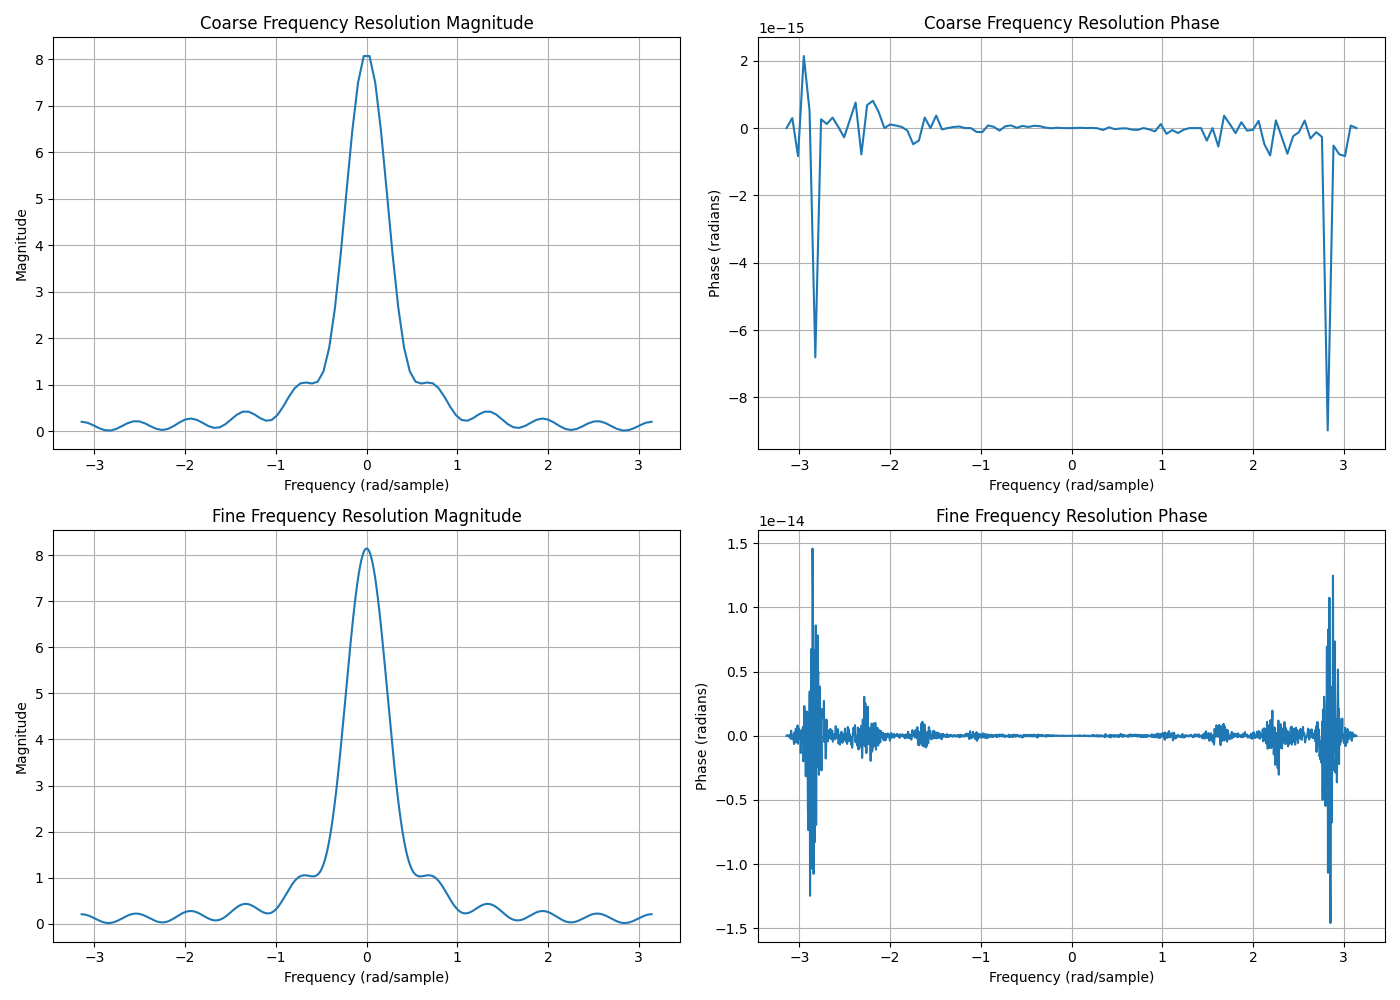
\includegraphics[width=\textwidth]{fig/ex4_c_plot}
\caption{Magnitude and phase of DTFT - coarse and fine}
\label{fig:ex4_c_plot}
\end{figure}

